% Created 2019-02-05 火 17:40
% Intended LaTeX compiler: pdflatex
\documentclass[11pt]{article}
\usepackage[utf8]{inputenc}
\usepackage[T1]{fontenc}
\usepackage{graphicx}
\usepackage{grffile}
\usepackage{longtable}
\usepackage{wrapfig}
\usepackage{rotating}
\usepackage[normalem]{ulem}
\usepackage{amsmath}
\usepackage{textcomp}
\usepackage{amssymb}
\usepackage{capt-of}
\usepackage{hyperref}
\date{}
\title{}
\hypersetup{
 pdfauthor={},
 pdftitle={},
 pdfkeywords={},
 pdfsubject={},
 pdfcreator={Emacs 26.1 (Org mode 9.1.9)}, 
 pdflang={Jp}}
\begin{document}

\setcounter{tocdepth}{3}
\tableofcontents


\section{序論}
\label{sec:orga5fc43d}
\subsection{背景}
\label{sec:org2c0cb16}
A City is Not a Tree
知識はツリー構造ではない.
code開発における文書管理は高度に発達しつつある.なぜなら,多くの開発者が共同で作業をするため,文書を管理することは開発,また情報を共有していく上で必要不可欠である.
しかし,中には文書を作った後に手を加えることなく放置することや,共有することなく個人でのみ管理してしまう場合もある.


\subsubsection{Sphinx}
\label{sec:org46bbe60}
Sphinxは, python製のドキュメント作成ツールである. reStructuredText記法が用いられており,LaTexやjupyter notebookと同様に,HTML, PDFなどに変換が可能なツールである.
Sphinxの最大の特徴は, 構造化に3つのレベルが存在することである.

\paragraph{レベル1 1つのファイル内の構造化}
\label{sec:orga48b90e}
テキストはツリー構造を持ち, reStructuredTextで書かれた文章は構造化され, 見た目にもわかりやすい体裁となっている.
文章が構造化されていると, 各情報が同列であるのか, 親子構造であるのか明確になり, 組み替えや並び替えが容易となる利点がある.

\paragraph{レベル2 ファイルとディレクトリの構造化}
\label{sec:org7dc4f6f}
ドキュメントの規模が大きくなると, ファイルとディレクトリで文章を分割し構造化する. 分割元から分割先へは親子関連付けを持たせることでツリー構造を維持する.
また, ファイルが多くなるとファイルをグループ化しディレクトリで階層化することで構造化を進める.

\paragraph{レベル3 ネットワークの構造化}
\label{sec:org48145d6}
ドキュメントに記載するキーワードや別の章へのポインタを一定のルールで持たせることで, Wikiのような柔軟なネットワーク構造を作る.
このように, 構造化の3レベルにWikiのようなネットワークのみのセミラティス構造とは異なり, ツリー構造を基本としている.

\subsection{目的}
\label{sec:org834ec2f}
文書を作成する際,易しく,わかりやすい文書を書くことができれば,仕事の成果も上がり,技術者としての信用も増すのではないでしょうか.[SEのための「構造化」文書作成の技術, p16]
毎週のレポート,学期末試験,卒業論文のように文書作成は規模が大きくなるに連れて破綻する.
文書やdirectoryがツリー構造に捉われることなく,呼び出すことが理想である.
そこでファイル構造をセミラティス構造にすることにより,規模が大きくなったとしても「ファイルが見つかりません」や「リンク切れ」を防ぐことができる.
また,文書をwebに公開する際にlinkの問題が発生する.
それらを解決するために,webで公開できる場合(webに掲載済み),できない場合(ジャーナルや本の内容)に場合分けを行い,
参照の付け替え(linkを本のタイトルに変更する等)を行うか否かを選択することで,link問題を解決する.


\subsubsection{ツリー構造}
\label{sec:org62ade77}

\subsubsection{セミラティス構造}
\label{sec:orgbfd7c98}
セミラティス構造とは, 1965年にウィーン出身の建築家であるクリストファー・アレグザンダーによって発表された論文''A City is Not a Tree''で考案された構造である. アレグザンダーは, セミラティス構造とツリー構造の違いを, 整数の集合$\backslash${1, 2, 3, 4, 5, 6$\backslash$}をどのように分類するのかという事例'''図''' を用いて説明した. 図1では, 部分集合として$\backslash${1, 2, 3$\backslash$},$\backslash${3, 4$\backslash$}, $\backslash${4, 5$\backslash$}, $\backslash${2, 3, 4$\backslash$}, $\backslash${3, 4, 5$\backslash$}, $\backslash${1, 2, 3, 4, 5$\backslash$}, $\backslash${3, 4, 5, 6$\backslash$}が存在する. このように, グループ同士に, 重複が生じる構造をセミラティス構造という. 一方で, ツリー構造では, グループ同士が重複することなく綺麗に分離されている構造である.


\subsubsection{テクニカルライティング}
\label{sec:org220a029}
テクニカルライティングとは,科学技術情報を正確かつ効果的に伝達するための文書作成技法のことである.

\paragraph{テクニカルライティングの効用}
\label{sec:org864c6fd}
\begin{enumerate}
\item わかりやすい説明により,ユーザの使い勝手が良くなる.
\item マニュアル作成の品質向上や効率向上ができ,開発工数が少なくなる.
\item ユーザからの問い合わせやクレームが少なくなる.
[SEのための「構造化」文書作成の技術, p26 - p27]
\end{enumerate}

\subsection{手法}
\label{sec:orgfd1967c}

\subsubsection{org}
\label{sec:org3f57bfc}

この図\ref{fig:orga757cce}のように

\begin{figure}[htbp]
\centering
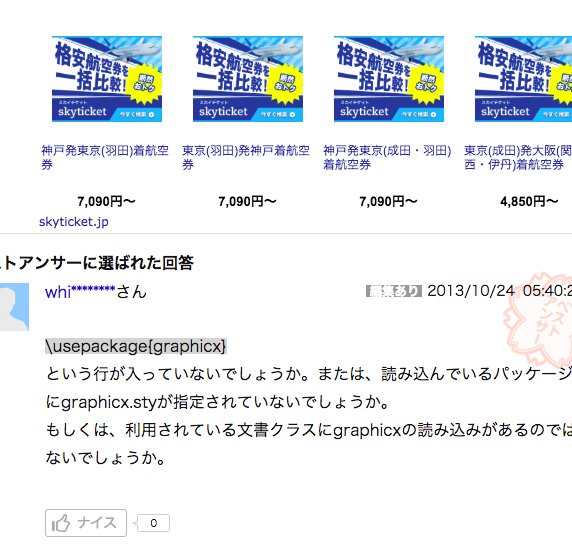
\includegraphics[width=5cm]{./test2.png}
\caption{\label{fig:orga757cce}
図の下につける名前}
\end{figure}

\subsubsection{Jupyter Notebook}
\label{sec:orge2e897a}

\subsubsection{RubyGems}
\label{sec:orgd3974eb}

\subsubsection{Thor}
\label{sec:org4e58ec6}

\subsubsection{Github}
\label{sec:org6542729}

\subsection{ornbの概要}
\label{sec:orgf828505}
\end{document}
